\section{Rekonstruktion}

In diesem Abschnitt werden die einzeln Schritte zum Rekonstruieren der Korrespondenzen erklärt, die im vorherigen Prozess gebildet worden sind. 
Für die Rekonstruktion wird die Klasse \emph{SceneReconstructor} in der Datei \emph{reconstruction.hpp} definiert und in \emph{reconstruction.cpp} implementiert. 
Die Klasse besitzt einen Konstruktor, welche eine Instanz der Calibration Klasse als Argument benötigt. 
Mit der Instanz wird die private Member-Variable \emph{calbiration} instanziiert, so dass sie später bei manchen Berechnungen verwendet werden kann.
Des Weiteren wird öffentlich die Methode \emph{reconstructScenes} definiert.
Diese Methode erfordert eine Instanz der Iterator-Klasse mit dem ImagePair als Template-Type. %TODO: check spelling
Mit dem Iterator werden in der Methode die korrespondierenden Bildpunkte rekonstruiert.
Dabei wird darauf geachtet, dass die rekonstruierten Punkte der einzelnen Paare später auch zusammen passen.
Wie in XXX zusehen ist, werden einige weitere private Methoden für die Klasse definiert.
Diese werden in den folgend Paragraphen erläutert, wenn sie für bestimmte Berechnungen genutzt werden.

Die Rekonstruktion wird mit den folgenden 5 Schritten durchgeführt:

\begin{enumerate}
    \item Lokale Rotation \& Translation bestimmen
    \item globale Translation berechnen
    \item Projektionsmatrix berechnen
    \item Triangulation
    \item Skalieren
        \begin{enumerate}
            \item skalierte globale Translation berechnen
            \item Projektionsmatrix berechnen
            \item Triangulation
        \end{enumerate}
\end{enumerate}

Im ersten Schritt muss für ein Bildpaar die Rotation und Translation der einen Kamera bestimmt werden.
Dazu kann wie in \cref{sec:essential-matrix} beschrieben wird, die essentielle Matrix berechnet und in $R$ und $t$ zerlegt werden.
OpenCV bietet dafür die Funktionen \emph{findFundamentalMat} und \emph{recoverPose} an.
In Zeile XXX des Listings XXX wird findFundamentalMat aufgerufen. 
Hier bei werden die korrespondierenden Bildpunkte der beiden Bilder und die Kalibrierungsmatrix übergeben.
Mit den weiteren drei Argumenten wird der angewendete Algorithmus gewählt und angepasst.
Mit dem Literal \emph{cv::RANSAC} wird der Ransac Algorithmus gewählt und so angepasst, das mit 99.9\% Wahrscheinlichkeit die bestimmte Matrix korrekt ist.
Als Threshold für Punkte, die innerhalb der essentielle Matrix passen, wir 1 Pixel verwendet. 
Neben Ransac kann auch LMED verwendet werden.
Der Grundlegende Unterschied der beiden Algorithmen ist XXX.
Es wird Ransac verwendet weil XXX.
Mit dem Mask Argument, wird in einem Vektor vermerkt, welche der Matches Ausreißer sind.
Die somit bestimmte essentielle Matrix wird dann in Zeile XXX mit recoverPose zerlegt.
Dazu werden neben der essentiellen Matrix auch die wieder die korrespondierenden Bildpunkte und die Kalibrierungsmatrix angegeben.
% erkläre kurz die Methode

Die zuvor berechnete Rotationsmatrix und Translationsvektor beschreiben nur die Ausrichtung und der Verschiebung der rechten Kamera im Vergleich zur linken Kamera.
Die Punkte, die mit dieser Pose rekonstruiert werden, werden in einem Koordinatensystem beschrieben, dessen Zentrum und Ausrichtung durch die linke Kamera definiert wird.
Dies gilt für jedes Bildpaar in der Sequenz, d.h.\ jedes Bildpaar definiert ihr eigenes Koordinatensystem.
Damit alle rekonstruierten Bildpunkte im gleichen Koordinatensystem dargestellt werden, müssen $R$ und $t$ transformiert werden.
Die Transformation des nten Bildpaars kann die mit 
\[ T_n = T_{n-1} \cdot \begin{bmatrix}
            R & t \\
            0 & 1 \\
        \end{bmatrix}
    \] 
berechnet werden.
Dabei ist $T_0$ die $4 \times 4$ Identitätsmatrix.
Die Transformationsmatrix $T_n$ kann nun in $R_n$ und $t_n$ aufgeteilt werden. 
$R_n$ und $t_n$ sind hierbei die Rotation und Translation der rechten Kamera des nten Bildpaares im Bezug auf die linke Kamera des ersten Paars.
Es gilt $T_n = \begin{bmatrix}
                R_n & t_n \\
                0 & 1 \\
            \end{bmatrix}$
Für diesen Schritt wird in XXX Zeile XXX die Methode \emph{combineToTranformation} implementiert.
Sie nimmt als Argumente eine $3 \times 3$ und eine $1\times3$ Matrix an und erstellt mit ihnen eine 
$4\times4$ Transformationsmatrix.
Die Transformationsmatrix des vorherigen Bildpaares $T_{n-1}$ wird von der Methode \emph{getPreviousTransform} der ImagePair Klasse bereit gestellt.
Ihre Implementation kann in XXX nachgeschaut werden.
Die Methode \emph{getFromTransformation} in XXX ist eine Hilfsmethode zum Extrahieren der Rotation und Translation einer $4\times4$ Transformationsmatrix.

Mit $R_n$ und $t_n$ wird in Schritt 4 mit der Formel XXX die Projektionsmatrix berechnet.
Die Berechnung wird durch die Methode \emph{getProjection} durchgeführt.
Wie in XXX zu sehen ist, werden nur die Rotation und Translation als Argumente benötigt.
Die Kalibrierungsmatrix $K$ wird durch die Instanz der Calibraion Klasse bereitgestellt. 

Die Schritte 2 und 3 werden in einer Methode zusammengefasst, da sie im vierten Schritt wiederholt werden müssen.
Dazu wird in XXX die Methode \emph{computePoseAndProjection} implementiert, die $T_n$ und die Projektionsmatrix zurück gibt.

In Schritt 4 werden die Bildpunkte mit der Methode \emph{triangulatePoints} von Opencv rekonstruiert.
Sie benötigt als Argumente die Projektionsmatrizen beider Kameras, sowie die Korrespondenzen aus beiden Bilder.  
Zurückgegeben wird eine $4\times N$ Opencv Matrix, die die rekonstruierten Punkte in homogenen Koordinaten repräsentiert.
Hier kommt noch was genaueres

Die Rekonstruktion des ersten Bildpaares ist mit diesem Schritt bereits vollendet.
Durch die Methode \emph{setReconstruction} werden die Ergebnisse der Rekonstruktion für die aktuelle ImagePair Instanz gespeichert.
Dieser Methode werden die Projektionsmatrix, die Transformationsmatrix, die rekonstruierten Punkte und die Maske der Ausreißer als Argumente übergeben. 
Wie in XXX zusehen ist, werden die Projektions- und Transformationsmatrix einfach den Member-Variablen zugewiesen.
Die rekonstruierten Punkte werden dahingegen gefiltert und zu einem vector<cv::Point3f> konvertiert.
Dabei werden alle Ausreißer, die in der notiert sind, und alle Punkte, die einen negativen Wert für ihre Z-Koordinate haben.  
Grund dafür ist, dass die Richtung der Kameras in Richtung der Z-Achse definiert ist.
Ein Punkt mit negativer Z-Achse liegt also hinter der Kamera, was physikalisch unmöglich ist und daher gefiltert werden muss.
Die Punkte liegen in homogenen Koordinaten vor, weswegen jeder Punkt vor dem Filtern durch das vierte Element geteilt werden muss.
Somit haben alle Punkte den gleichen Faktor 1.
Gleichzeitig wird die Map \emph{matchIdxToWorldPoint} aufgebaut.
Sie bildet den Index der korrespondierenden Bildpunkten des Bildpaares auf den Index des dadurch rekonstruierten Punkt ab.
Diese Abbildung wird benötigt, um im fünften Schritt die Skalierung durchführen zu können.

Im fünften und letzten Schritt wird die Skalierung für das aktuelle Bildpaar bestimmt, damit alle Punkte mit dem selben Maßstab rekonstruiert werden.  
Dazu werden die Abstände der rekonstruierten Punkte aus dem vorherigen Bildpaar mit den Abständen der rekonstruierten Punkte des aktuellen Paars verglichen.
Es muss hierbei darauf geachtet werden, dass die verwendeten Punkte des vorherigen Paars jeweils Korrespondenzen im aktuellen Bild haben.
Die Abbildung \cref{fig:sfm-scaling} illustriert diesen Zusammenhang.
Mit dem Verhältnis der Abstände, kann der Translationsvektor $t$ entsprechend skaliert werden.


Bevor die Skalierung bestimmt werden kann, werden die rekonstruierten Punkte normalisiert und gefiltert.
Gleichzeitig werden die Indizes der nicht Ausreißer in einem Vektor gespeichert. 
Die Indizes werden benötigt, um mit der Methode \emph{getMatchingWorldPoints} der ImagePair Klasse die rekonstruierten Punkte des vorherigen Paars zu bestimmen.
Für jeden jedes Feature Match werden die entsprechenden Indizes der linken und rechten Bildpunkte in den Member-Variablen gespeichert.
Die Indizes der Bildpunkte des linken Bilds wird der Methode \emph{getMatchingWorldPoints} übergeben, die auf die Instanz des vorherigen Bildpaars angewendet wird.
Es ist somit möglich die korrespondierenden Matches und die damit verbundenen Weltpunkte zu bestimmen.
Anschließend werden Paare der Weltpunkte des vorherigen Paars und den respektiven Weltpunkten des
aktuellen Bildpaars.
Die Distanz zwischen den jeweiligen Paaren werden als Vektorbetrag berechnet.
Die Skalierung für das aktuelle Bildpaar ist das Mittel aller Distanzverhältnisse.
Der Translationsvektor $t$ wird mit der Skalierung multipliziert und es werden die Schritte 2 bis 5 wiederholt.
Zum Schluss kann wird die Methode \emph{setReconstruction} aufgerufen, um die skalierten Weltpunkte zu speichern.
\begin{figure}
    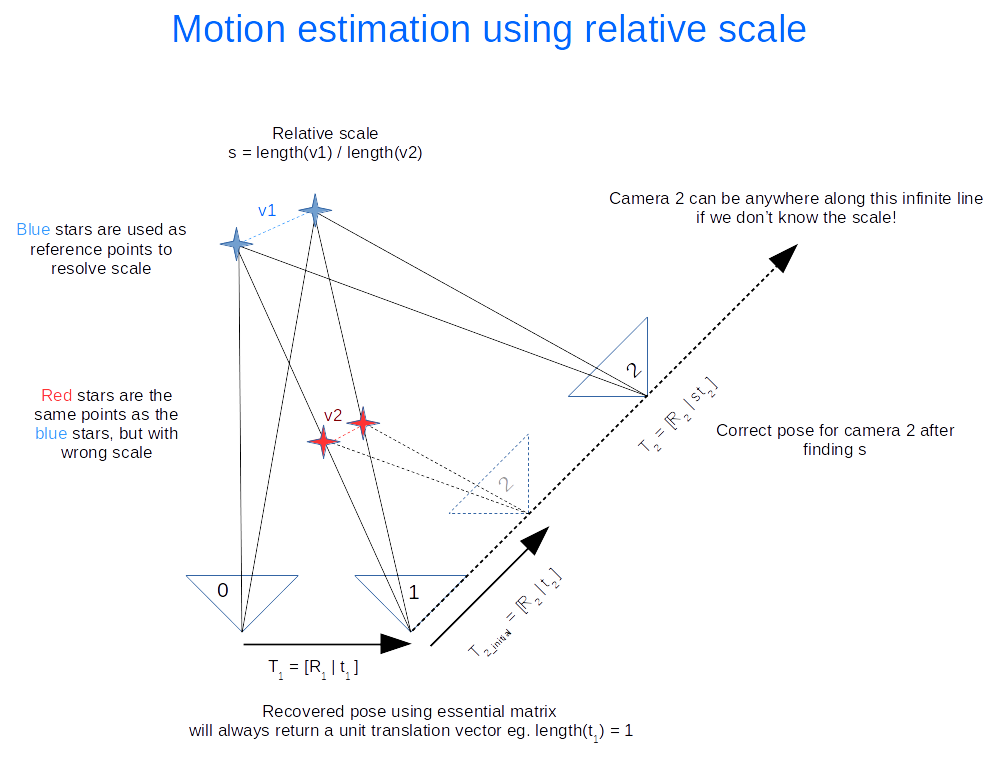
\includegraphics[width=\textwidth]{src/img/nghiaho_2017_sfm_scaling}
    \caption{~\cite{nghiaho_2017}}
    \label{fig:sfm-scaling}
\end{figure}
